\section{Thiết kế Cơ sở dữ liệu}

Dữ liệu được tổ chức dưới dạng Document (MongoDB). Dưới đây là chi tiết các Schema:

% ---------------------------------------------------------
% 1. USER SCHEMA
% ---------------------------------------------------------
\subsection{User Schema}
Schema này lưu trữ thông tin tài khoản và hồ sơ người dùng.

\begin{figure}[H]
    \centering
    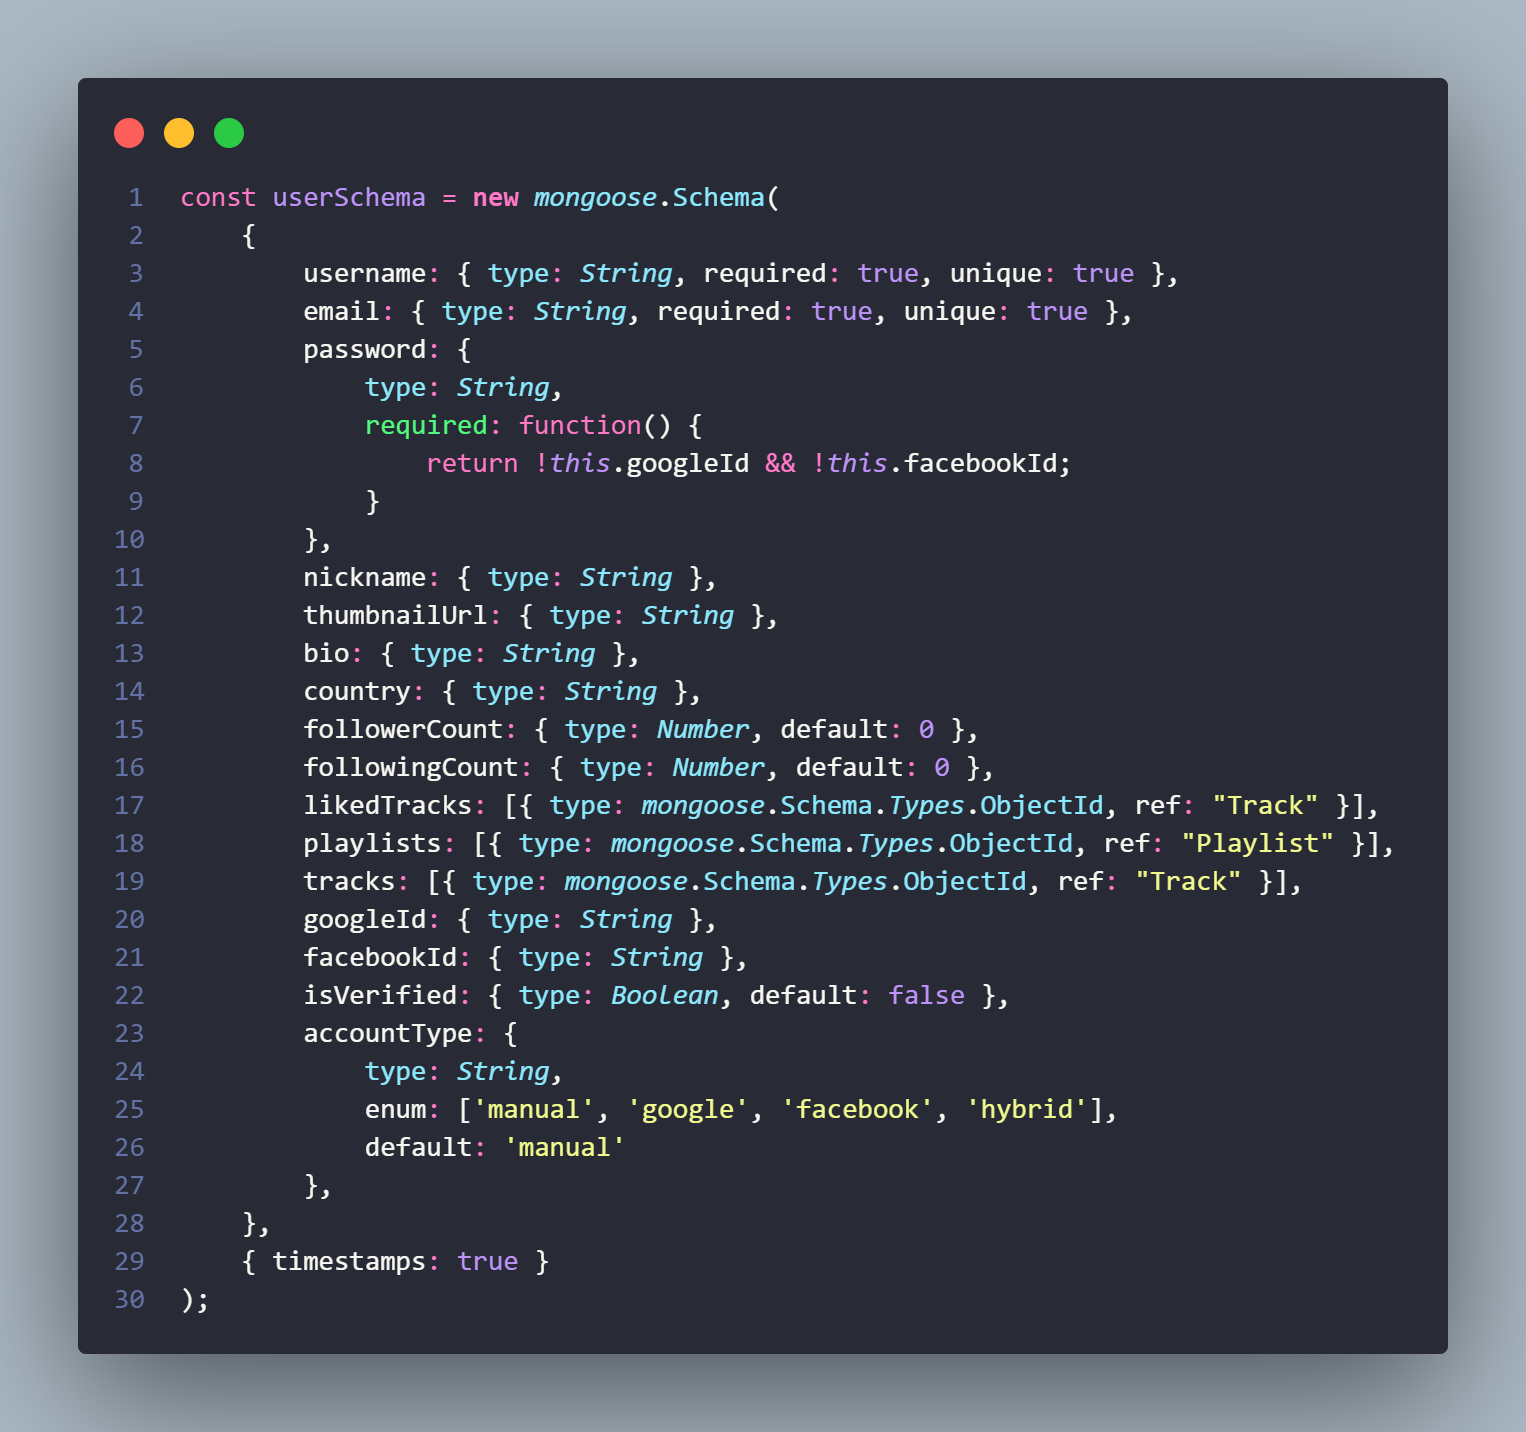
\includegraphics[width=0.9\textwidth]{Images/schema/userSchema.png} 
    \caption{Sơ đồ User Schema}
\end{figure}

\begin{longtable}{|c|l|p{9cm}|}
    \hline
    \textbf{STT} & \textbf{Trường} & \textbf{Mô tả} \\ \hline
    % \endfirsthead
    % \hline
    % \textbf{STT} & \textbf{Trường} & \textbf{Mô tả} \\ \hline
    % \endhead
    % \hline
    % \endfoot
    
    1 & username & Tên đăng nhập duy nhất của người dùng \\ \hline
    2 & email & Địa chỉ email duy nhất \\ \hline
    3 & password & Mật khẩu (bắt buộc nếu không dùng Google/Facebook) \\ \hline
    4 & nickname & Tên hiển thị của người dùng \\ \hline
    5 & accountType & Loại tài khoản (manual, google, facebook, hybrid) \\ \hline
    6 & isVerified & Trạng thái xác thực tài khoản (Boolean) \\ \hline
    7 & followerCount & Số lượng người theo dõi \\ \hline
    8 & followingCount & Số lượng người đang theo dõi \\ \hline
\end{longtable}

% ---------------------------------------------------------
% 2. TRACK SCHEMA
% ---------------------------------------------------------
\subsection{Track Schema}
Schema lưu trữ thông tin về bài hát được tải lên hệ thống.

\begin{figure}[H]
    \centering
    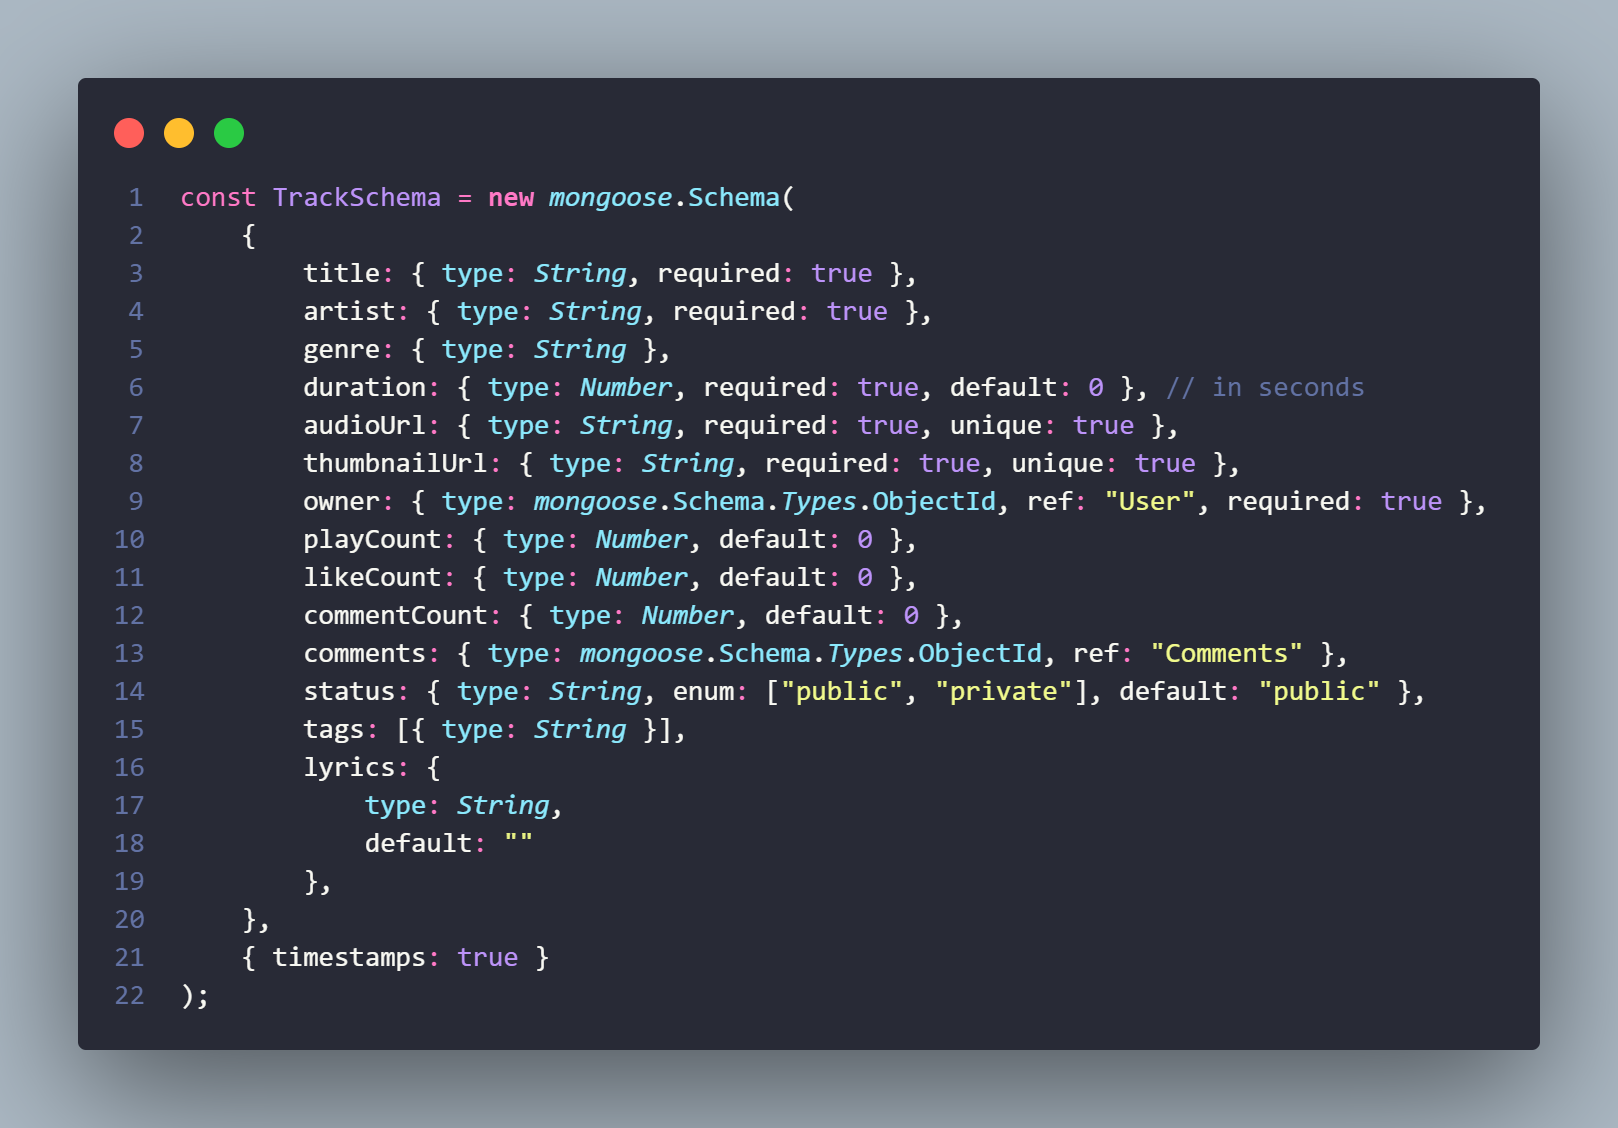
\includegraphics[width=0.9\textwidth]{Images/schema/trackSchema.png}
    \caption{Sơ đồ Track Schema}
\end{figure}

\begin{longtable}{|c|l|p{9cm}|}
    \hline
    \textbf{STT} & \textbf{Trường} & \textbf{Mô tả} \\ \hline
    1 & title & Tên bài hát \\ \hline
    2 & artist & Tên nghệ sĩ thể hiện \\ \hline
    3 & audioUrl & Đường dẫn đến file âm thanh gốc \\ \hline
    4 & thumbnailUrl & Đường dẫn ảnh bìa bài hát \\ \hline
    5 & owner & ID người dùng (User) tải bài hát lên \\ \hline
    6 & status & Trạng thái hiển thị (public/private) \\ \hline
    7 & lyrics & Lời bài hát \\ \hline
    8 & playCount & Tổng số lượt phát \\ \hline
    9 & likeCount & Tổng số lượt thích \\ \hline
    10 & comments & Danh sách comments \\ \hline
\end{longtable}

% ---------------------------------------------------------
% 3. PLAYLIST SCHEMA
% ---------------------------------------------------------
\subsection{Playlist Schema}
Schema lưu trữ thông tin danh sách phát nhạc.

\begin{figure}[H]
    \centering
    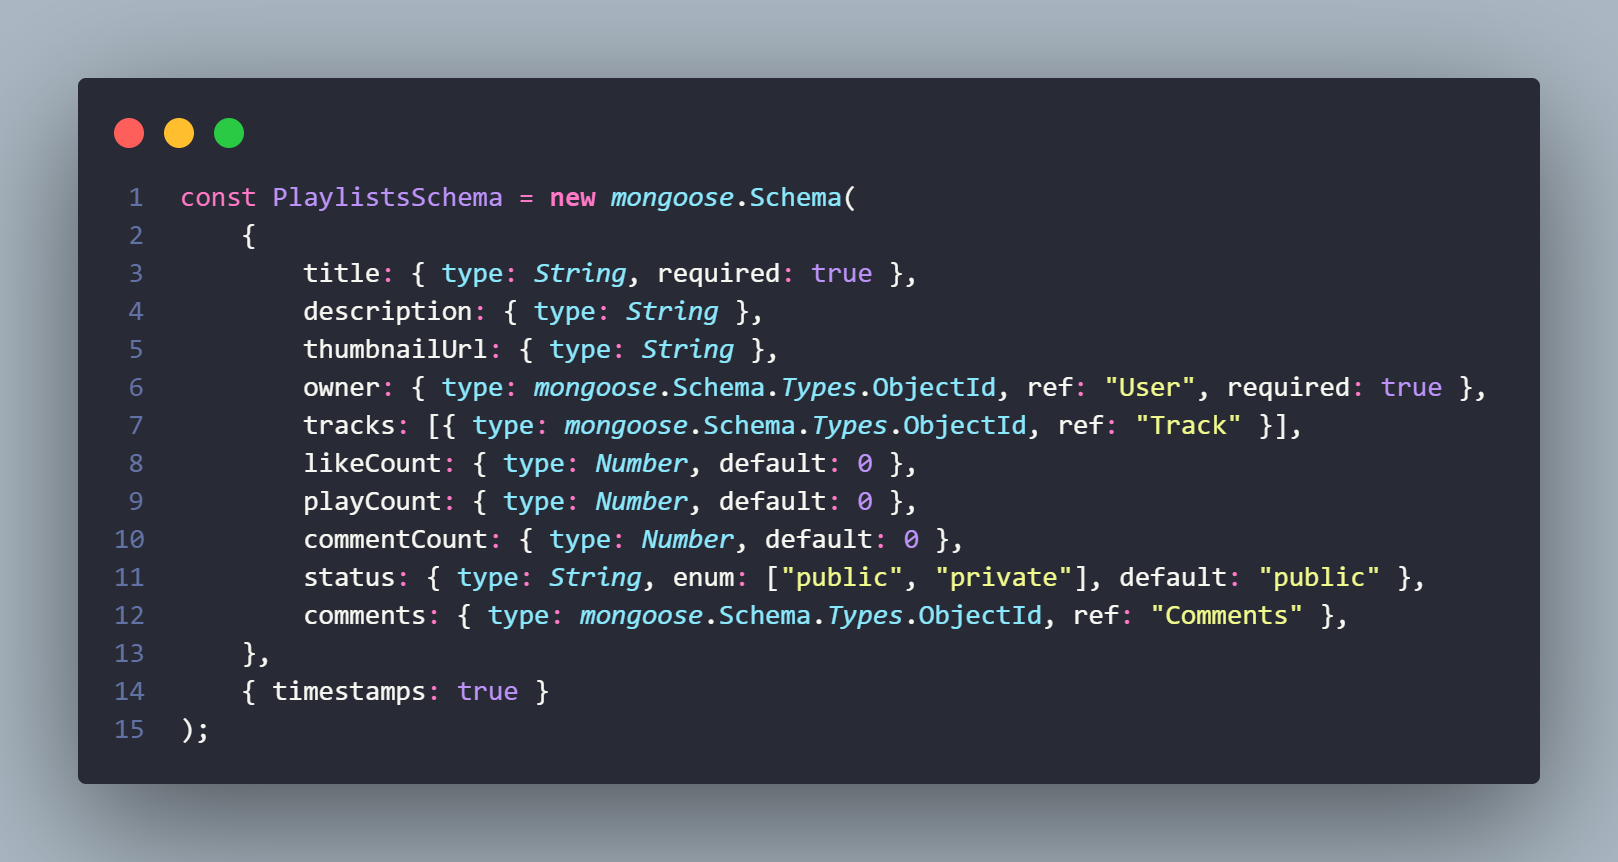
\includegraphics[width=0.9\textwidth]{Images/schema/playlistSchema.png}
    \caption{Sơ đồ Playlist Schema}
\end{figure}

\begin{longtable}{|c|l|p{9cm}|}
    \hline
    \textbf{STT} & \textbf{Trường} & \textbf{Mô tả} \\ \hline
    1 & title & Tên danh sách phát \\ \hline
    2 & description & Mô tả ngắn về danh sách phát \\ \hline
    3 & owner & ID người sở hữu danh sách phát \\ \hline
    4 & tracks & Mảng chứa ID các bài hát (Track) trong playlist \\ \hline
    5 & status & Trạng thái công khai hoặc riêng tư \\ \hline
    6 & likeCount & Số lượt thích playlist \\ \hline
    7 & thumbnailUrl & Đường dẫn ảnh bìa danh sách phát \\ \hline
\end{longtable}

% ---------------------------------------------------------
% 4. NOTIFICATION SCHEMA
% ---------------------------------------------------------
\subsection{Notification Schema}
Schema quản lý các thông báo gửi đến người dùng.

\begin{figure}[H]
    \centering
    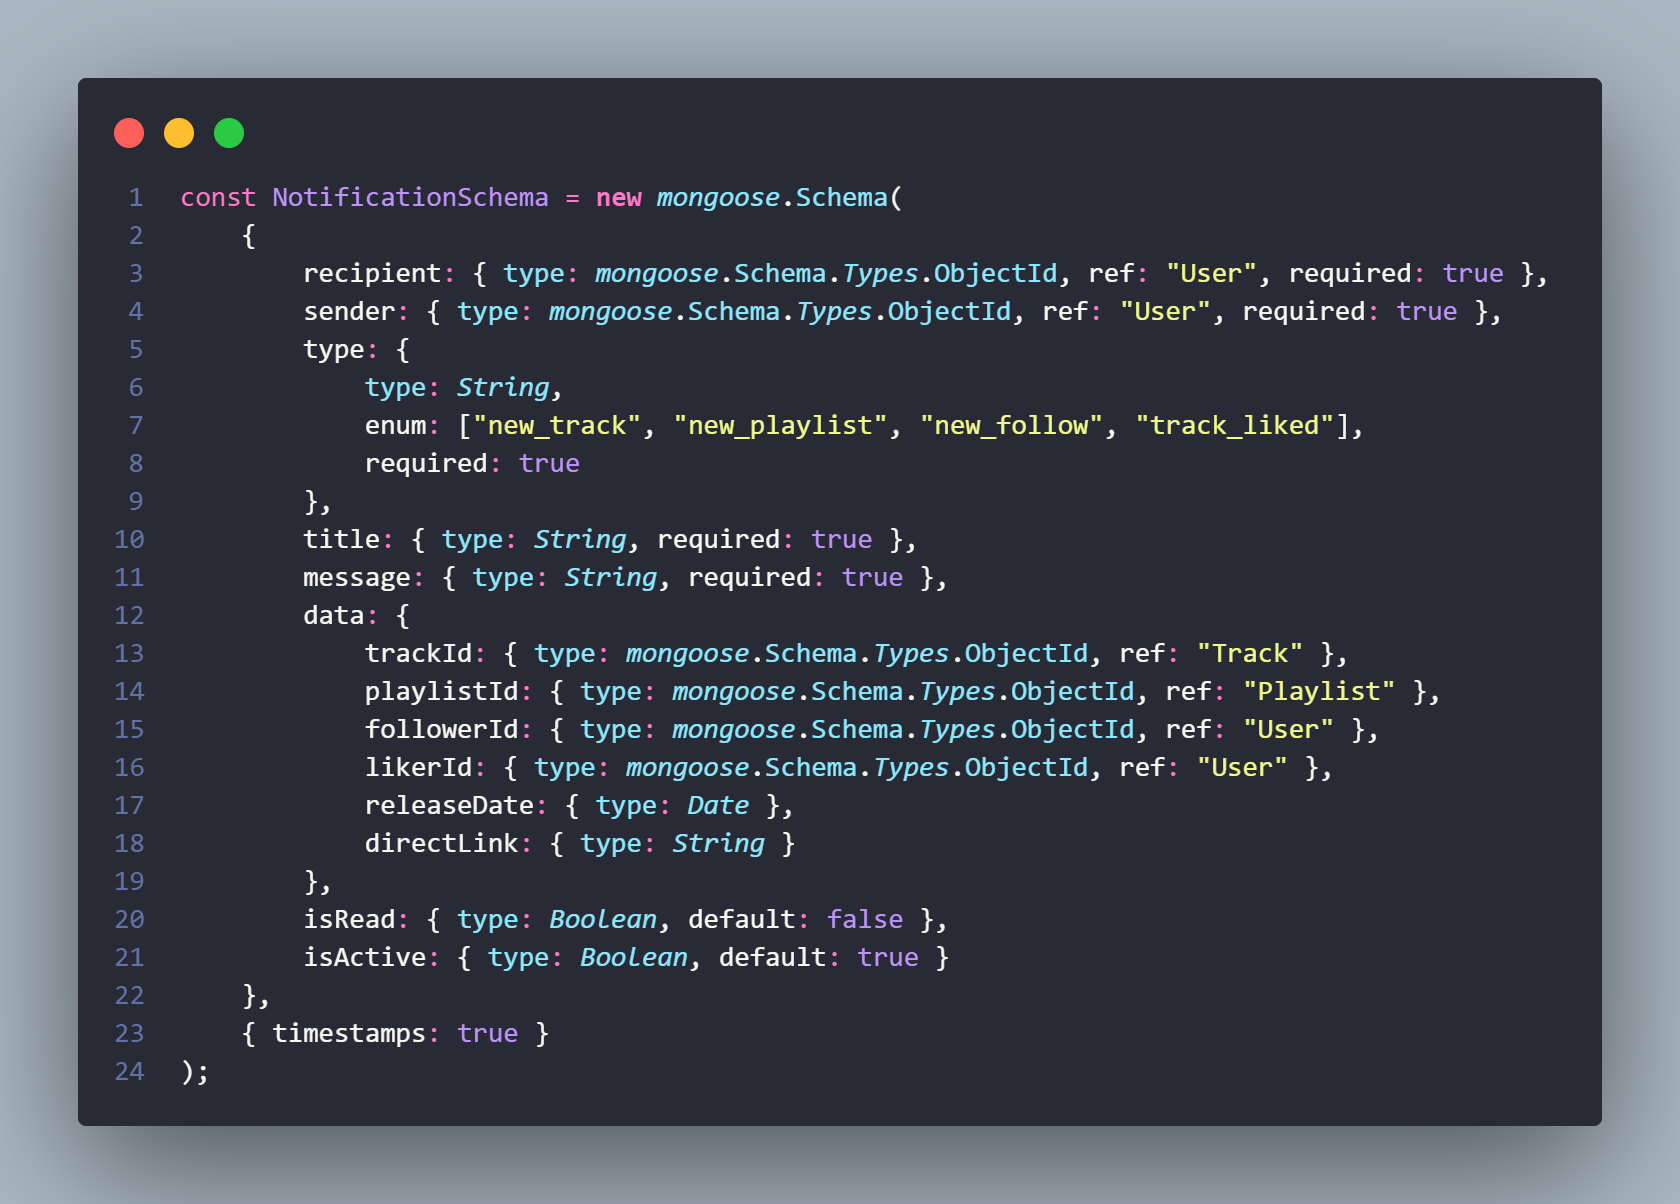
\includegraphics[width=0.9\textwidth]{Images/schema/notificationSchema.png}
    \caption{Sơ đồ Notification Schema}
\end{figure}

\begin{longtable}{|c|l|p{9cm}|}
    \hline
    \textbf{STT} & \textbf{Trường} & \textbf{Mô tả} \\ \hline
    1 & recipient & ID người nhận thông báo \\ \hline
    2 & sender & ID người gửi thông báo \\ \hline
    3 & type & Loại thông báo (new\_track, new\_follow, v.v.) \\ \hline
    4 & message & Nội dung hiển thị của thông báo \\ \hline
    5 & isRead & Trạng thái đã đọc (Boolean) \\ \hline
    6 & data & Object chứa ID liên quan (trackId, playlistId...) \\ \hline
\end{longtable}

% ---------------------------------------------------------
% 5. COMMENT SCHEMA
% ---------------------------------------------------------
\subsection{Comment Schema}
Schema quản lý các bình luận của người dùng.

\begin{figure}[H]
    \centering
    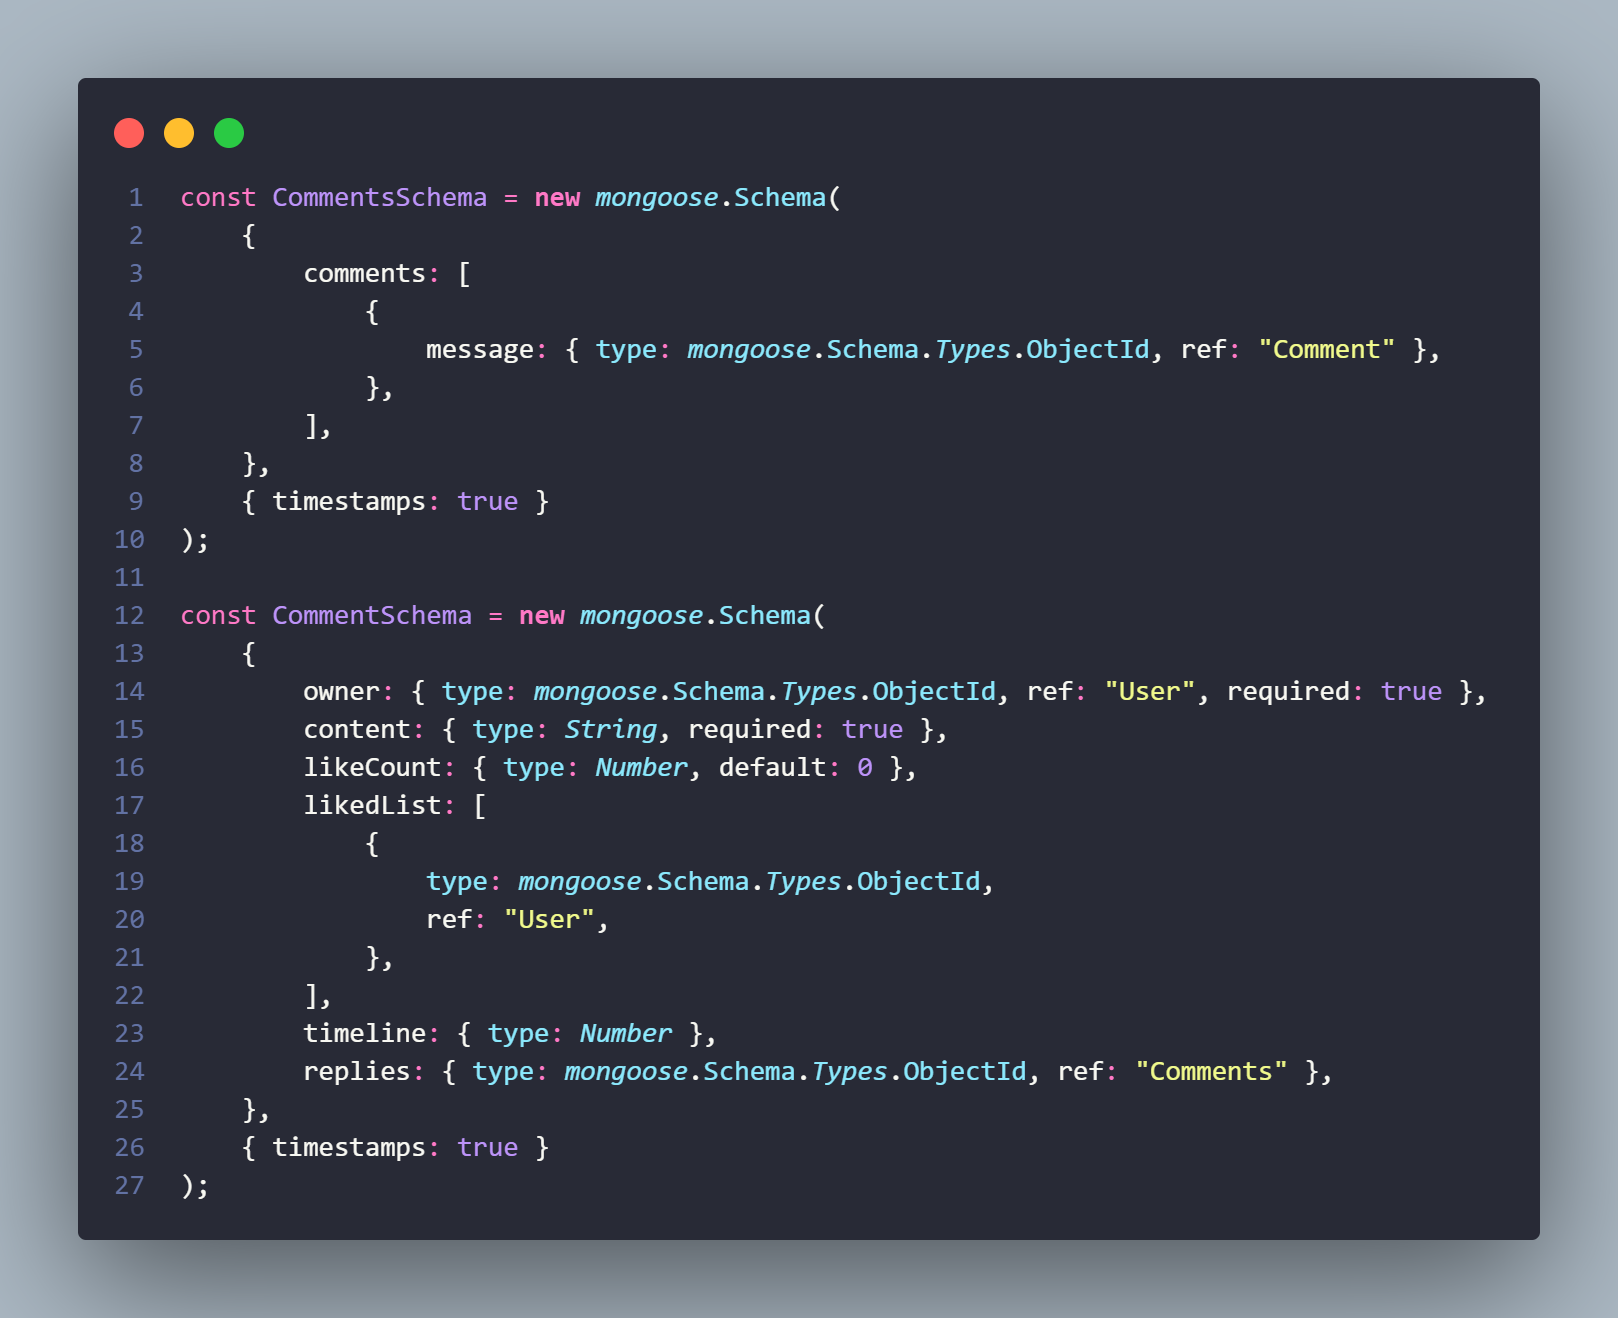
\includegraphics[width=0.9\textwidth]{Images/schema/commentSchema.png}
    \caption{Sơ đồ Comment Schema}
\end{figure}

\begin{longtable}{|c|l|p{9cm}|}
    \hline
    \textbf{STT} & \textbf{Trường} & \textbf{Mô tả} \\ \hline
    1 & owner & ID người viết bình luận \\ \hline
    2 & content & Nội dung bình luận \\ \hline
    3 & likeCount & Số lượt thích của bình luận \\ \hline
    4 & replies & ID tham chiếu đến các câu trả lời (nested comments) \\ \hline
    5 & timeline & Thời điểm bình luận trong bài hát (giây) \\ \hline
\end{longtable}

% ---------------------------------------------------------
% 6. FOLLOW SCHEMA
% ---------------------------------------------------------
\subsection{Follow Schema}
Schema quản lý mối quan hệ theo dõi giữa người dùng.

\begin{figure}[H]
    \centering
    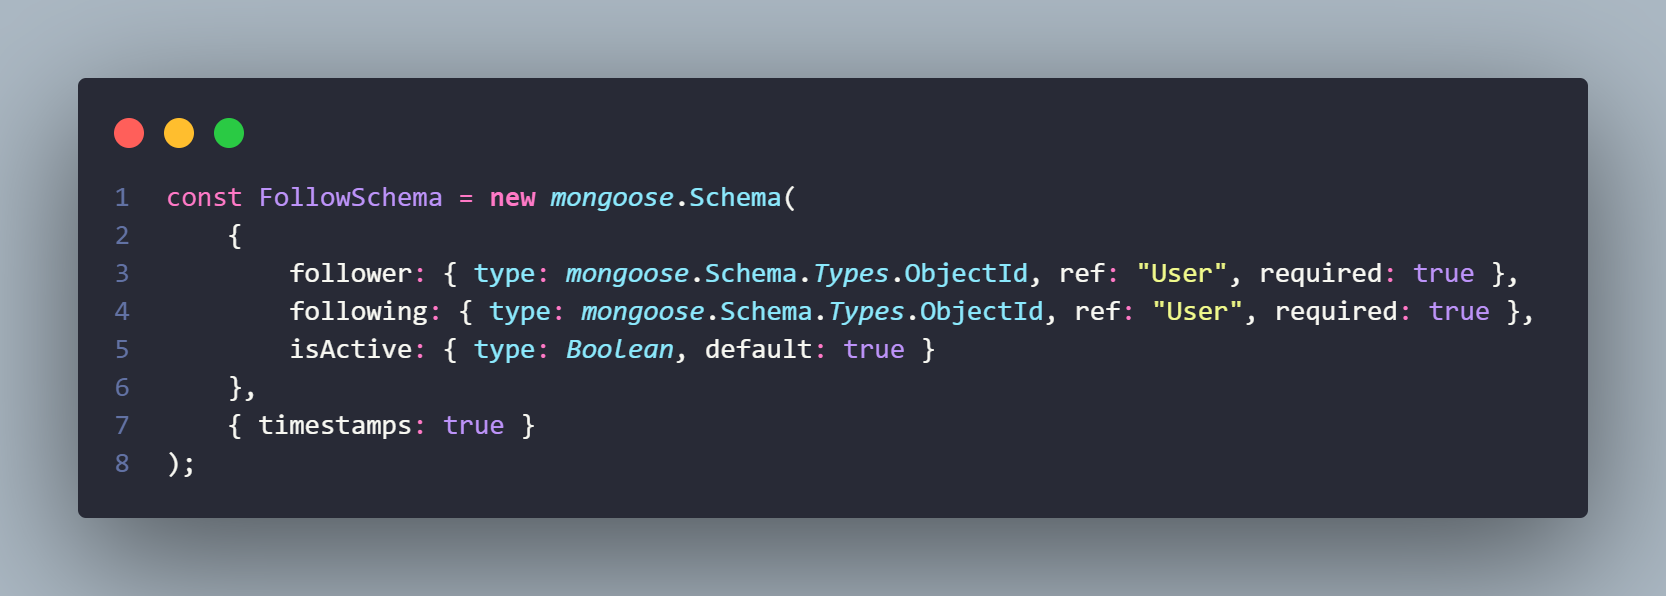
\includegraphics[width=0.9\textwidth]{Images/schema/followSchema.png}
    \caption{Sơ đồ Follow Schema}
\end{figure}

\begin{longtable}{|c|l|p{9cm}|}
    \hline
    \textbf{STT} & \textbf{Trường} & \textbf{Mô tả} \\ \hline
    1 & follower & ID người theo dõi \\ \hline
    2 & following & ID người được theo dõi \\ \hline
    3 & isActive & Trạng thái hoạt động của mối quan hệ \\ \hline
\end{longtable}